\documentclass[11pt]{article}
\usepackage{cs170}
\usepackage{tikz}
\usepackage{pgfplots}
\usetikzlibrary{tikzmark}
\usepackage{tikz-qtree}
\usepackage{tabularx}

\newcommand{\circled}[2]{%
    \tikz[baseline=(char.base)]{\node[draw, circle, inner sep=1pt] (char) {#1};}%
    }

\def\title{Homework 8}
\def\duedate{3/18/2024, at 10:00 pm (grace period until 11:59pm)}

\begin{document}
\maketitle

Due \textbf{\duedate}

\question{Study Group}
List the names and SIDs of the members in your study group.
If you have no collaborators, you must explicitly write ``none''.

\begin{solution} I worked on this homework with the following collaborators:
\begin{itemize}
    \item Lakshya Nagal, SID: 3037935253
\end{itemize}
\end{solution}

\question{Faster Longest Increasing Subsequence}

Recall the dynamic programming algorithm for LIS from lecture. It has the recurrence, 
\[
    L[i] = \max_{j < i : A[j] < A[i]} L[j]+1,
\]
where $L[i]$ is the length of the longest increasing subsequence that includes and ends at $A[i]$. Using DP to compute all the $L[i]$'s takes $O(N^2)$ time, where $N$ is the length of the array $A$. In this problem, we will see how to reformulate the problem so that we can use binary search to obtain a $O(N\log N)$ time algorithm.
% For simplicity we will assume that all the elements of $A$ are distinct.

Consider the following subproblem definition:
\[M_i[j] = \text{the smallest element that ends any subsequence of length $j$ for $A[1 \dots i]$}.\]

where $M_i$ is 1-indexed. 

We can set $M_i[k]=\infty$ if no increasing subsequence of length $k$ exists in $A[1\dots i]$.

\begin{subparts}
    \subpart Given the following array of length $10$, compute the values of $M_8$. Recall that $M_8$ only considers the elements $A[1\dots 8]$. What is the length of the LIS of $A[1\dots 8]$, and what is the last element of the LIS?
    \begin{table}[htbp]
        \centering
        \begin{tabular}{|c|c|c|c|c|c|c|c|c|c|}
            \hline
            5 & 3 & 7 & 4 & 1 & 2 & 5 & 7 & 8 & 3 \\
            \hline
        \end{tabular}
    \end{table}\\
    \begin{solution}
        \begin{align*}
            M_8[1] &= [5], [3], [7], [4], [1], [2], [5], [7] \rightarrow \circled{1}{}\\
            M_8[2] &= [5, 7], [3, 7], [3, 4], [4, 5], [4, 7], [1, 2], [1, 5], [1, 7], [2, 5], [2, 7] \rightarrow \circled{2}{}\\
            M_8[3] &= [3, 4, 5], [3, 4, 7], [3, 5, 7], [4, 5, 7], [1, 2, 5], [1, 5, 7], [2, 5, 7] \rightarrow \circled{5}{}\\
            M_8[4] &= [3, 4, 5, 7], [1, 2, 5, 7] \rightarrow \circled{7}{}\\
            M_8[5] &= M_8[6] = M_8[7] = M_8[8] = \infty
        \end{align*}
        $M_8 = [1, 2, 5, 7, \infty, \infty, \infty, \infty]$\\
        The longest subsequence is $4$ and the last element is \circled{7}{}.
    \end{solution}
    \subpart Show that $M_i$ is a strictly increasing array, i.e. that $M_i[j] < M_i[j+1]$ for all $j = 1, \dots, N - 1$.

    \emph{Hint: Suppose there exists some $j$ such that $M_i[j] \geq M_i[j+1]$, and show that this implies a contradiction.}\\
    \begin{solution}
        Suppose there is some $j$ such that $M_i[j]=e_j, M_i[j+1] = e_{j+1}$ where $e_j \geq e_{j+1}$. By definition $e_j, e_{j+1}$ are the 
        smallest elements that end any subsequence of length $j$ and $j+1$ respectively. Because $e_j$ is the smallest element in any subsequence of length $j$, then
        this implies that for any subsequence of length $j+1$, $e_j$ occurs before $e_{j+1}$ in the array, meaning that $e_j < e_{j+1}$, contradicting our initial assumption.
    \end{solution}
    \subpart Given the same array as part (a), compute $M_{10}$.\\
    \begin{solution}
        \begin{align*}
            M_{10}[1] &= [5], [3], [7], [4], [1], [2], [5], [7], [8], [3] \rightarrow \circled{1}{}\\
            M_{10}[2] &= [5, 7], [5, 8], [3, 7], [3, 4], [3, 5], [3, 8], [7, 8], [4, 5], [4, 7], [4, 8], [1, 2], [1, 5], [1, 7], [1, 8],\\ 
                   &~~~~   [1, 3], [7, 8] \rightarrow \circled{2}{}\\
            M_{10}[3] &= [5, 7, 8], [3, 7, 8], [3, 4, 5], [3, 4, 7], [3, 4, 8], [4, 5, 7], [4, 5, 8], [4, 7, 8], [1, 2, 5], [1, 2, 7],\\
                   &~~~~ [1, 2, 8], [1, 5, 7], [1, 7, 8], [1, 2, 3], [2, 5, 7], [2, 5, 8], [2, 7, 8], [5, 7, 8] \rightarrow \circled{3}{}\\
            M_{10}[4] &= [3, 5, 7, 8], [3, 4, 5, 1], [3, 4, 5, 8], [3, 5, 7, 8], [4, 5, 7, 8], [1, 2, 5, 7], [1, 2, 5, 8], [1, 2, 7, 8],\\
                   &~~~~ [1, 5, 7, 8], [2, 5, 7, 8]\rightarrow \circled{7}{}\\
            M_{10}[5] &= [1, 2, 5, 7, 8], [3, 4, 5, 7, 8] \rightarrow \circled{8}{}\\
            M_{10}[6] &= M_{10}[7] = M_{10}[8] = M_{10}[9] = M_{10}[10] = \infty
        \end{align*}
        $M_{10} = [1, 2, 3, 7, 8, \infty, \infty, \infty, \infty, \infty]$
    \end{solution}
    \subpart Let $j$ be the smallest index such that $M_i[j] \geq A[i + 1]$. Prove that the length of the LIS ending on $A[i + 1]$ is $j$. \\
    \emph{Hint: Use the result from (b) to show that there exists a length $j$ increasing subsequence ending on $A[i+1]$, and that there exist no longer increasing subsequence.}\\
    \begin{solution}
        Given that $M_i[j] \geq A[i + 1]$ we know that there exist an increasing subsequence of length $j-1$ ending at some element
        where $M_i[j-1] < A[i+1]$. If we include the $A[i+1]$ element to this subsequence we end up with an increasing 
        subsequence of length $j$ ending at A[i+1]. Showing that indeed the length of the LIS ending at $A[i+1]$ is $j$.
        % Suppose there exist an increasing subsequence greater than $j$ ending at $A[i+1]$, then this implies that 
        % there would be an increasing subsequence of length $j$ ending at some value smaller than $A[i+1]$. contradicting the 
        % assumption that $j$ is the smallest index such that $M_i[j] \geq A[i+1]$.
    \end{solution}
    \subpart Now show that only one element differs between $M_i$ and $M_{i+1}$. Recall that $M_i$ only accounts for $A[1 \dots i]$, so we are trying to prove $M_{i+1}$ can be computed for $A[1 \dots i+1]$ by taking $M_i$ and modifying one element.\\
    \begin{solution}
        When we transition from $M_i$  to $M_{i+1}$, we are essentially including the element $A[i+1]$ to the set.
        Concluding that with the addition of $A[i+1]$, $M_i$ and $M_{i+1}$ differ by at most one element.
    \end{solution}
    \newpage
    \subpart Now combining the previous subparts, write pseudocode that finds the longest increasing subsequence of an array $A$ in $O(N \log N)$ time. 
    
    \emph{Hint: a naive implementation using the 2D subproblem $M_i[j]$ would still yield a runtime of $O(N^2)$. To achieve the $O(N \log N)$ runtime, you only need to store a single 1D array $M$. Then, efficiently update $M$ by using previous subparts.}\\
    \begin{solution}
        \begin{verbatim}
            def longest_increasing_subsequence(A):
                n = len(A)
                M = [0] * (n+1)
                M[0] = 0
                parents = [0] * (n+1)
                l = 0

                for i in range(n):
                    lo, hi = 0, l
                    while lo <= hi:
                        mid = (lo + hi) // 2
                        if M[mid] < A[i]:
                            low = mid+1
                        else:
                            hi = mid-1
                    M[lo] = A[i]
                    parents[i] = M[lo-1]

                lis = [0] * (l)
                k = M[l]
                for i in range(0, n, -1):
                    if A[i] = k:
                        lis[l] = A[i]
                        l -= 1
                    k = parent[i]
                return lis
        \end{verbatim}
        \begin{itemize}
            \item We iterate over every element of $A$ and run binary search to find the largest index $j$
            such that $M[j] \le A[i]$. Then we update M and parents (holds the indices of the elements that are part of the LIS).
            \item Starting at the last index of $A$, we trace back through parents to reconstruct LIS.
        \end{itemize}
    \end{solution}
\end{subparts}

\newpage

\question{Max Independent Set Again}

You are given a connected tree $T$ with $n$ nodes and a designated root $r$, where every vertex $v$ has a weight $W[v]$. A set of nodes $S$ is a $k$-independent set of $T$ if $|S| = k$ and no two nodes in $S$ have an edge between them in $T$. The weight of such a set is given by adding up the weights of all the nodes in $S$, i.e. 
\[W(S) = \sum_{v \in S} W[v].\] Given an integer $k \leq n$, your task is to find the maximum possible weight of any $k$-independent set of $T$. We will first tackle the problem in the special case that $T$ is a binary tree, and then generalize our solution to a general tree $T$.

\begin{subparts}
    \item Assume that $T$ is a binary tree, i.e. every node has at most 2 children.  Describe an $O(nk^2)$ algorithm that solves this special case, and analyze its runtime. Proof of correctness and space complexity analysis are not required.\\
    \begin{solution}
        Let $I_1(v, s)$ be the maximum weight of the independent set of size $s$ with its root at $v$. Let $I_2(u, s)$ be the maximum 
        weight of the independent set of size $s$ rooted at $u \in children(v)$. Lets consider the case
        where $v$ is included in the set. If $v$ is included in the set, then we have the following recurrence:\\
        \begin{align*}
            I_1(v, s) = max\{I_2(v_L, s') + I_2(v_R, s-s')\}
        \end{align*}
        This recurrence skips over the children of $v$ since it was chosen and we consider new subproblems where $s'$ is the size the new subset given by all possible sizes less than s. 
        The next recurrence arises from skipping over $v$, in this case we consider $u \in children(v)$:
        \begin{align*}
            I_2(u, s) = max\begin{cases}
                            I_1(u, s), \text{if we skip over $u$}\\
                            max\{W[u] + I_1(u_L, s') + I_1(u_R, s-s')\}, \text{if we choose $u$}
                        \end{cases}
        \end{align*}
        For both recurrences, subscripts $R$ and $L$ denote the right and left children of a vertex.\\
        For our base cases we have $I_1(v, 0) = 0$ and $I_2(u, 0) = 0$
       \\\textbf{Runtime: }There are $O(nk)$ subproblems each bounded by $O(k)$ to solve, for a total of $O(nk^2)$
    \end{solution}
    \newpage
    \item Now, consider any arbitrary tree $T$, with no restrictions on the number of children per node. Describe how we can add up to $O(n)$ ``dummy'' nodes (i.e. nodes with weight 0) to $T$, as well as some edges, to convert it into a binary tree $T_b$. \\
    \begin{solution}
        Consider the following tree:
        \tikzset{every tree node/.style={minimum width=1em,draw,circle},
            blank/.style={draw=none},
            edge from parent/.style=
            {draw,edge from parent path={(\tikzparentnode) -- (\tikzchildnode)}},
            level distance=1.2cm}
            \begin{center}
                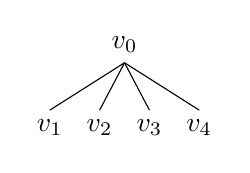
\begin{tikzpicture}
                    \Tree
                    [.$v_0$     
                        [
                            .$v_1$ 
                        ]
                        [
                            .$v_2$
                        ]
                        [
                            .$v_3$
                        ]
                        [
                            .$v_4$
                        ]
                    ]
                \end{tikzpicture} \\
            \end{center}
            Ignoring the left most child, we can add dummy nodes as follows:
            \begin{center}
                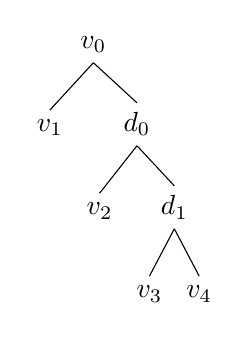
\begin{tikzpicture}
                    \Tree
                    [.$v_0$     
                        [
                            .$v_1$ 
                        ]
                        [
                            .$d_0$ 
                            \edge[];
                                [
                                    .$v_2$
                                ]
                            \edge[];
                                [
                                    .$d_1$
                                    \edge[];
                                    [
                                        .$v_3$
                                    ]
                                    [
                                        .$v_4$
                                    ]
                                ]
                        ]
                    ]
                \end{tikzpicture}
            \end{center}
            If $|children(v_0)| > 2$, then we can take the right most two children and add dummy node $d$, as the parent of the two 
            children, then add this dummy node as a child of $v_0$ Where $W[d] = 0$. We recursively do this until $|children(v_0)|=2$. Adding up to $O(n)$ dummy nodes.
    \end{solution}
    \newpage
    \item Describe an $O(nk^2)$ algorithm to solve the general case (i.e. when $T$ is any arbitrary tree), and analyze its runtime. Proof of correctness and space complexity analysis are not required.

    \emph{Hint: there exists two ways (known to us) to solve this. One way is to combine parts (a) and (b), and then modify the recurrence to account for the dummy nodes. The other way involves 3D dynamic programming, in which you directly extend your recurrence from part (a) to iterate across vertices' children. We recommend the first way as it may be easier to conceptualize, but in the end it is up to you!}\\
    \begin{solution}
        We begin by turning $T$, into a binary tree $T'$as seen in (b) which gives us the runtime $O(n)$, we then proceed to use the algorithm
        from part (a) to solve the problem, using $T'$. The recurrence from part (a) has to be updated to account for 
        the dummy nodes. we can do this by adding a new case to our recurrences, that states that if we are at a dummynode, we skip it and
        consider the children of the dummy node, using the same recurrence as from part (a). 
    \end{solution}
\end{subparts}

\newpage

\question{Canonical Form LP}
Recall that any linear program can be reduced to a more constrained \emph{canonical form} where all variables are non--negative, the constraints are given by $\leq$ inequalities, and the objective is the maximization of a cost function. 

\noindent More formally, our variables are $x_i$. Our objective is $\max c^\top x = \max \sum_i c_i x_i$ for some constants $c_i$. The $j$th constraint is  $\sum_i a_{ij} x_i \leq b_j$ for some constants $a_{ij}, b_j$. Finally, we also have the constraints $x_i \geq 0$.

\noindent An example canonical form LP: 
\begin{center}
$\mbox{ maximize } 5x_1 + 3x_2$
\begin{align*}
\text{subject to } \begin{cases} x_1 + x_2 - x_3 \leq 1 \\
-(x_1 + x_2 - x_3) \leq -1 \\
-x_1 + 2x_2 + x_4 \leq 0 \\ 
-(-x_1 + 2x_2 + x_4) \leq 5 \\
x_1, x_2, x_3, x_4 \ge 0
\end{cases}
\end{align*}
\end{center} 

\noindent For each of the subparts below, describe how we should modify it to so that it satisfies canonical form. If it is impossible to do so, justify your reasoning. 

Note that the subparts are independent of one another. Also, you may assume that variables are non-negative unless otherwise specified.
\begin{subparts}
  \subpart Min Objective: $\min \sum_i c_i x_i$\\
  \begin{solution}
    To turn the maximization problem into a minimization, just multiply the coefficients of the objective function by -1.
  \end{solution}
%   \hideifsol{\vspace{2cm}}
  \subpart Lower Bound on Variable: $x_1 \geq b_1$\\
  \begin{solution}
    In this situation we can multiply both sides by -1. $-x_1 \le -b_1$.
  \end{solution}
  \subpart Bounded Variable: $b_1 \leq x_1 \leq b_2$\\
  \begin{solution}
    We can re-write $b_1 \leq x_1 \leq b_2$ into $x_1 \le b_2$ and $x_1 \geq b_1$ then re-write $x_1 \geq b_1$ into
    $-x_1 \le -b_1$, so we have $b_1 \leq x_1 \leq b_2 \Leftrightarrow x_1 \le b_2, -x_1 \le -b_1$. 
  \end{solution}
  \subpart Equality Constraint: $x_2 = b_2$\\
  \begin{solution}
    We can re-write $x_2 = b_2$ into $x_2 \geq b_2$ and $x_2 \le b_2$ and re-write $x_2 \geq b_2$ into
    $-x_2 \le -b_2$ since $x_2 = b_2 \Leftrightarrow x_2 \le b_2, -x_2 \le -b_2$.
  \newpage
  \end{solution}
  \subpart More Equality Constraint: $x_1 + x_2 + x_3 = b_3$\\
  \begin{solution}
    We can re-write as:
    \begin{align*}
       x_1 + x_2 + x_3 &\le b_3\\
       x_1 + x_2 + x_3 \geq b_3 \Leftrightarrow -x_1 - x_2 - x_3 &\le -b_3
    \end{align*}
  \end{solution}
  \subpart Absolute Value Constraint: $|x_1+x_2| \leq b_2$ where $x_1, x_2 \in \R$\\
  \begin{solution}
    We can introduce new variables $y_1 = x_1 + x_2$ and $y_2 = - x_1 - x_2 \rightarrow -y_2 = x_1 + x_2$ and then re-write as:
    \begin{align*}
        y_1 &\le b_2 \\
        -y_2 &\le b_2
    \end{align*}
  \end{solution}
  \subpart Another Absolute Value Constraint: $|x_1 + x_2| \geq b_2$ where $x_1, x_2 \in \R$\\
  \begin{solution}
    Similar as above we introduce two non-negative variables $x^+, x^-$ and replace $x$ wherever it occurs 
    by $x^+-x^-$. So we have $x^+-x^- \geq b_2 \Leftrightarrow -x^{+} + x^{-} \le b_2$.
    % We can re-write as $y_1 = x_1 + x_2$ and $y_2 = -x_1 - x_2 \Rightarrow -y_2 = x_1 + x_2$ then re-write as:
    % \begin{align*}
    %     y_1 \geq b_2 \Leftrightarrow -y_1 &\le -b_2 \\
    %     -y_2 \geq b_2 \Leftrightarrow y_2 &\le -b_2
    % \end{align*}
  \end{solution}
  \subpart Min Max Objective: $\min \max (x_1,x_2,x_3,x_4)$
  \emph{Hint: use a dummy variable!}\\
  \begin{solution}`'
    Let $z = \max (x_1,x_2,x_3,x_4)$
    \begin{align*}
        \textbf{maximize: } -&z\\
        \textbf{Subject to: } &z \geq x_1\\
        &z \geq x_2\\
        &z \geq x_3\\
        &z \geq x_4
    \end{align*}
  \end{solution}

\end{subparts}

\newpage

\question{Baker}

You are a baker who sells batches of brownies and cookies (unfortunately no brookies... for now). Each brownie batch takes 4 kilograms of chocolate and 2 eggs to make; each cookie batch takes 1 kilogram of chocolate and 3 eggs to make. You have 80 kilograms of chocolate and 90 eggs. You make a profit of 60 dollars per brownie batch you sell and 30 dollars per cookie batch you sell, and want to figure out how many batches of brownies and cookies to produce to maximize your profits.

\begin{subparts}
\subpart Formulate this problem as a linear programming problem; in other words, write a linear program (in canonical form) whose solution gives you the answer to this problem. Draw the feasible region, and
find the solution using Simplex. \\
\begin{solution} Let $x_1$ be the number of brownie batches, and $x_2$ to the number of cookie batches.
    Additionally it is given that we make $\$60$/batch of brownies and $\$30$/batch of cookies which is what we want to maximize. Two other inequalities
    arise from the fact that we have limited ingredients.
    \begin{align*}
        \textbf{maximize: }& 60x_1 + 30x_2 \\
        \textbf{Subject to: }& 4x_1 + x_2 \leq 80 \quad \tikzmark{circle1} \\
        &2x_1 + 3x_2 \leq 90 \quad \tikzmark{circle2} \\
        &x_1 \geq 0\color{white}0 \quad \tikzmark{circle3} \\
        &x_2 \geq 0\color{white}0 \quad \tikzmark{circle4}
    \end{align*}
    \begin{tikzpicture}[overlay,remember picture]
        \node[draw, circle, inner sep=1.5pt] at ([xshift=1.45em,yshift=0.8ex]pic cs:circle1) {1};
        \node[draw, circle, inner sep=1.5pt] at ([xshift=1.0em,yshift=0.8ex]pic cs:circle2) {2};
        \node[draw, circle, inner sep=1.5pt] at ([xshift=4.2em,yshift=0.8ex]pic cs:circle3) {3};
        \node[draw, circle, inner sep=1.5pt] at ([xshift=4.2em,yshift=0.8ex]pic cs:circle4) {4};
    \end{tikzpicture}
    \begin{center}
        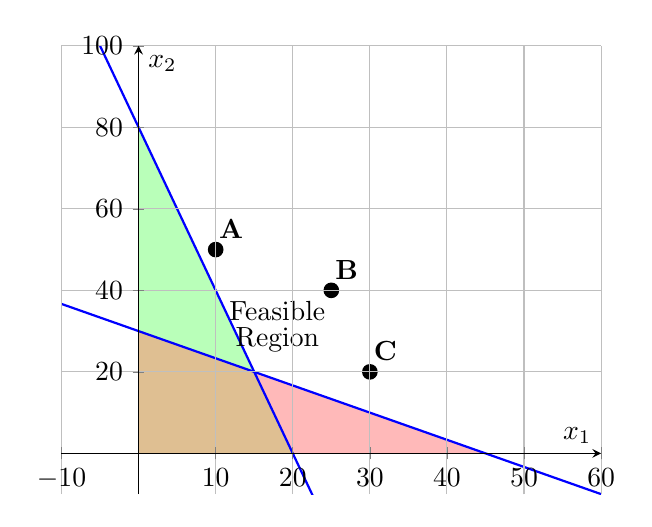
\begin{tikzpicture}
            \begin{axis}[
                xlabel={$x_1$},
                ylabel={$x_2$},
                xmin=-10, xmax=60,
                ymin=-10, ymax=100,
                axis lines=center,
                grid=both,
                axis on top,
                ]
                \addplot[smooth, dashed, blue] coordinates {(50, -10) (50, 100)};
                \addplot[smooth, dashed, blue] coordinates {(-10, 80) (100, 80)};
                \addplot[fill=green!55, draw=none, fill opacity=0.5] coordinates {(0, 0) (0, 80) (20, 0)};
                \addplot[fill=red!55, draw=none, fill opacity=0.5] coordinates {(0, 0) (0, 30) (45, 0)}; 
                \addplot[fill=yellow!55, draw=none, fill opacity=0.1] coordinates {(0,0) (0,30) (15,20) (20,0)};
                \addplot[smooth, thick, blue] coordinates {(-5, 100) (25, -20)}; %steep
                \addplot[smooth, thick, blue] coordinates {(-10, 36.667) (60, -10)};
                \node at (18, 35) {Feasible};
                \node at (18, 28) {Region};
                \node[circle,fill,inner sep=2pt] at (10, 50) {};
                \node[circle,fill,inner sep=2pt] at (25, 40) {};
                \node[circle,fill,inner sep=2pt] at (30, 20) {};
                \node at (27, 45) {\textbf{B}};
                \node at (12, 55) {\textbf{A}};
                \node at (32, 25) {\textbf{C}};
            \end{axis}
        \end{tikzpicture}
    \end{center}
    \centering \textbf{A}: (0, 30), \textbf{B}: (15, 20), \textbf{C}: (20, 0)\\
    After running simplex we arrive at the vertex given by equations \circled{1}{} and \circled{2}{} (from the re-written LP found during Simplex) since they satisfy the property $\forall_i c_i < 0$. After solving
    the system given by \circled{1}{} and \circled{2}{} from the original LP above, we get the optimal point \textbf{B} = $(15, 20)$, which gives us the solution $(60)(15) + (30)(20) = \$1500$ coming from baking 15 batches of brownies and 20 batches of cookies.
\end{solution}
\newpage
\subpart Suppose instead that the profit per brownie batch is $P$ dollars and the profit per cookie batch remains at 30 dollars. For each vertex you listed in the previous part, give the range of $P$ values for which that vertex is the optimal solution.\\
\begin{solution}
    We have $Px_1 + 30x_2$ and the points \textbf{A}: (0, 30), \textbf{B}: (15, 20), \textbf{C}: (20, 0).
    \begin{align*}
        \text{Point }\textbf{A}:(0, 30)\\
        P(0) + 30(30) &\geq 15P + 30(20)\\
        P(0) + 30(30) &\geq 20P + 30(0)\\
        \boxed{P \le 20}\\
        \text{Point }\textbf{B}: (15, 20)\\
        15P + 30(20) &\geq P(0) + 30(30)\\
        15P + 30(20) &\geq 20P + 0\\
        \boxed{20 \le P \le 120}\\
        \text{Point }\textbf{C}: (20, 0)\\
        P(20) + 30(0) &\geq P(0) + 30(30)\\
        P(20) + 30(0) &\geq 15P + 600\\
        \boxed{P \geq 120}
    \end{align*}
\end{solution}
\end{subparts}
\end{document}